\newpage
\chapter{Dataset}
\label{cha:dataset}

Most of the existing SISR methods are trained and evaluated on simulated datasets that assume simple and uniform degradation (i.e., bicubic degradation). Unfortunately, SISR models trained on such simulated datasets are hard to generalize for practical applications since the authentic degradations in real-world LR images are much more complex \cite{cai2019realworld}. Creating a large and varied enough dataset of real-world data with paired LR-HR images poses a challenge by itself, that being said the results of this research rely heavily on the quality of the data so a lot of work has gone into ensuring that the content of each pair of frames is consistent and reliable without sacrificing too many frames.

The main problems regarding the creation of the LR-HR pairs from two different cameras can be synthesized in:
\begin{itemize}
  \item different lens distortion
  \item spatial alignment
  \item temporal alignment
\end{itemize}

Focal length and Field of View are strongly related to each other. The Field of View (FOV) describes the physical area of the world that can be imaged on a sensor through a determined lens system, when described in degrees it's referred to as Angular FOV or AFOV.
The focal length of a lens is a fundamental parameter that describes how strongly it focuses or diverges light. A large focal length indicates that light is bent gradually while a short focal length indicates that the light is bent at sharp angles.
The focal length of a lens defines the AFOV, for a given sensor size, the shorter the focal length, the wider the AFOV. Additionally, the shorter the focal length of the lens, the shorter the distance needed to obtain the same FOV compared to a longer focal length lens \cite{flength}.

% \begin{wrapfigure}{l}{0.5\textwidth}
%   \begin{center}
%     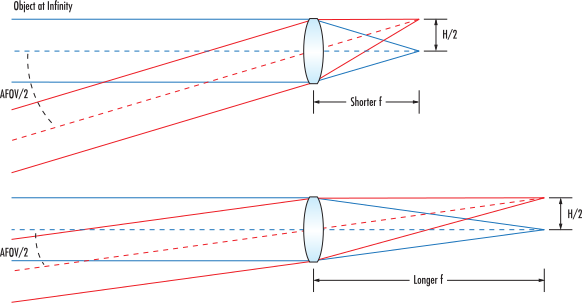
\includegraphics[width=0.48\textwidth]{figures/AFOV.png}
%   \end{center}
%   \caption{For a given sensor size H a longer focal length produces a larger AFOV}
% \end{wrapfigure}

\begin{figure}[h]
  \centering
  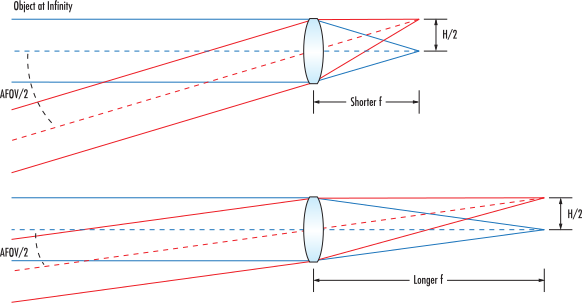
\includegraphics[scale=0.5]{figures/AFOV.png}
  \caption{For a given sensor size H a longer focal length produces a larger AFOV}
\end{figure}

The term distortion is often applied interchangeably with reduced image quality. However, distortion is an individual aberration that does not reduce the information in the image; most aberrations mix information together to create image blur, distortion simply misplaces information geometrically. This means that known distortion can be mapped or calculated and removed from an image, whereas information from other aberrations is lost and cannot easily be recreated.

Distortion is determined by the optical design of the lens. Lenses with larger FOVs will exhibit greater amounts of distortion, larger FOVs (a result of low magnification or short focal length) are more susceptible to distortion than smaller FOVs (high magnification or long focal length). The wide FOVs achieved by short focal length lenses must be weighed against the aberrations introduced to the system (such as distortion) \cite{distortion}.

\begin{figure}[h]
  \centering
  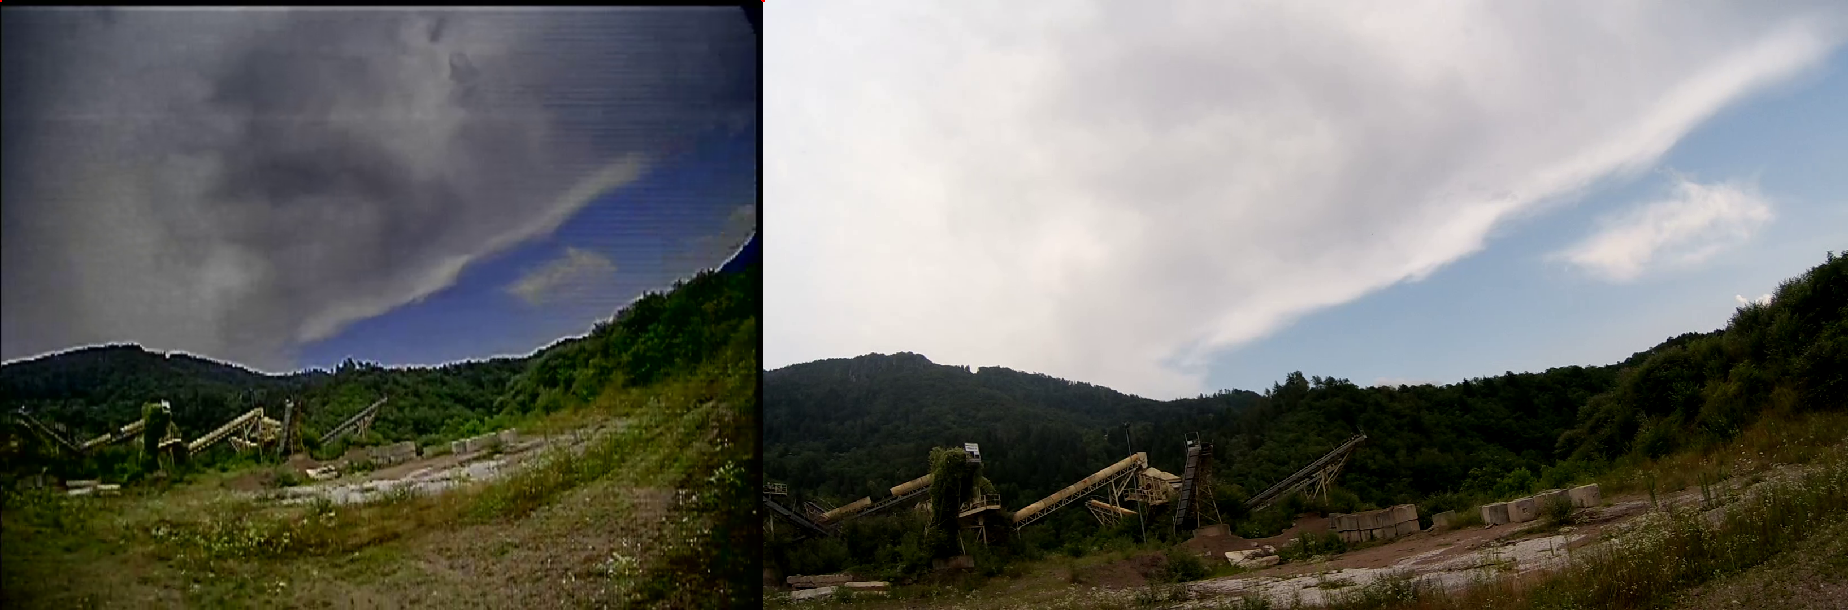
\includegraphics[width=1\textwidth]{figures/OG_sbs.png}
  \caption{Unprocessed LR and HR frames captured at the same instant}
  \label{img:og_sbs}
\end{figure}

As shown in Figure \ref{img:og_sbs} both images suffer from a great amount of distortion, it's especially noticeable on the sides of the image. A solution to this problem is to calibrate both cameras and use the obtained information to reproject all the image points without distortion.

Nevertheless removing the distortion is not enough, it's easy to see how the LR camera, with its shorter focal length and larger AFOV, captures a much larger angular section of the world compared to its HR counterpart, this is a spatial misalignment problem, but not the only cause. As explained previously both cameras are fixed in place, however, the entire rig is subject to strong vibrations caused by turbulences, high speed and the four motors spinning at tens of thousands of rounds per minute. All these vibrations cause the cameras to move slightly in all three axes, requiring further work in post-processing to get the images aligned.
It's been decided to ignore the parallax error produced by the distance between the cameras. In fact, the two sensors sit approximately at 2cm of distance which, thanks to the large AFOV, will only cause a sort of ”stereo” effect when subjects come close to the camera lenses, a situation that does not occur in the dataset: almost
all the subjects are positioned at several meters of distance. Therefore, the effect is barely detectable or missing completely.\newline

Another notable problem encountered during the dataset processing is temporal alignment. The cameras shoot respectively at 25fps and 60fps with shutter speeds of 1/50s and 1/120s. The result is that only a few frames end up capturing the same instant, with some partially overlapping and others starting at different times.

\begin{figure}[h]
  \centering
  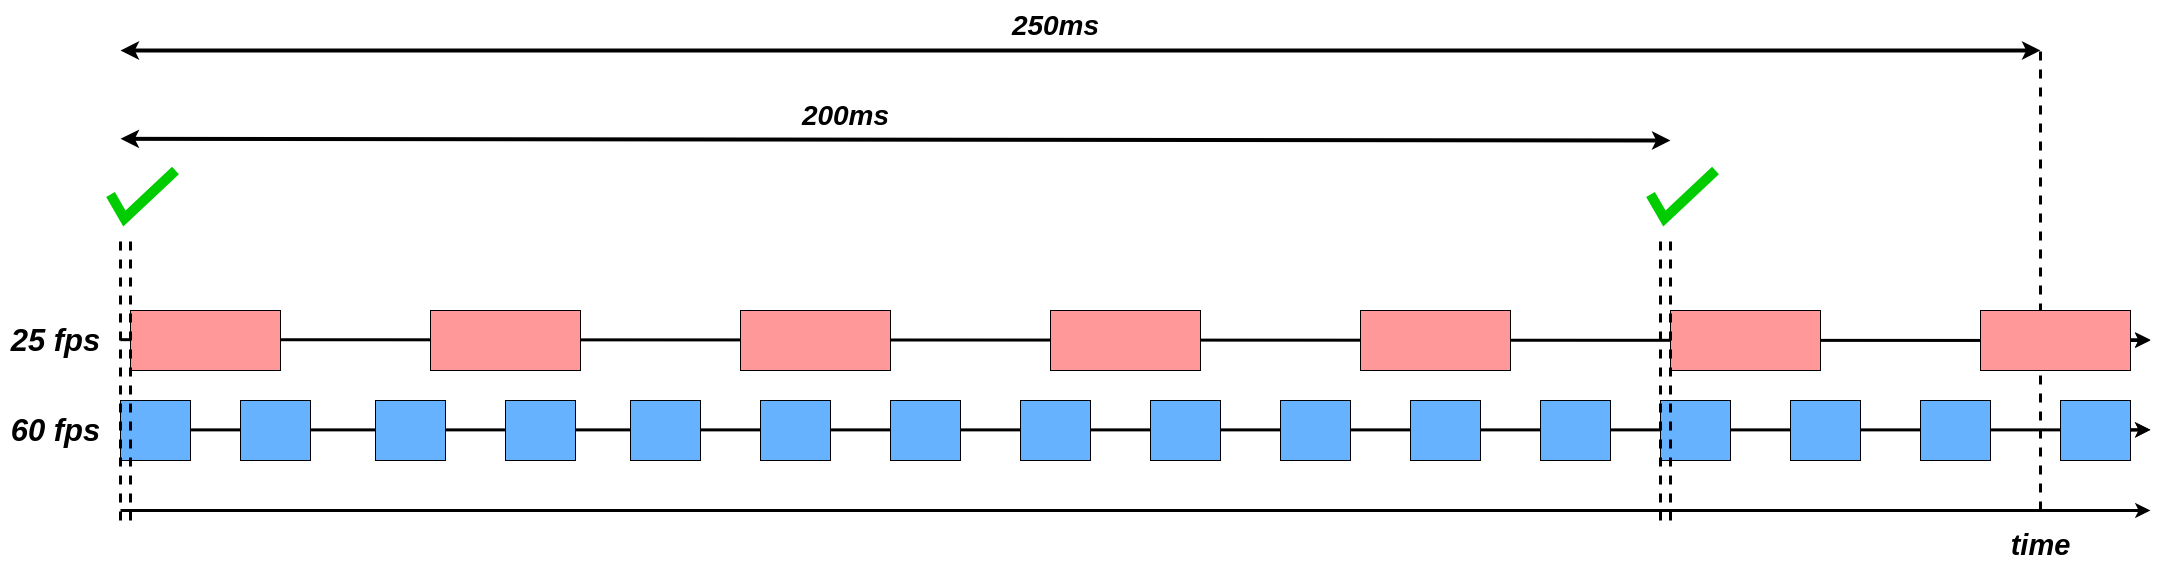
\includegraphics[width=1\textwidth]{figures/temporal_align_3.png}
  \caption{How frames are captured over the span of 1/4 of a second}
  \label{img:temp_align}
\end{figure}

As shown in Figure \ref{img:temp_align} only a handful of frames perfectly overlap and start capturing at the same moment. This turned out to be one of the main causes of missed alignment.
How these three problems have been tackled will be discussed in greater detail in chapters \ref{sec:camera_calib}, \ref{sec:temp_align} and \ref{sec:spatial_align}.

\section{Cameras}
\label{sec:cameras}

HR frames have been captured using a Runcam 2 \cite{runcam}, the digital camera offers to record at \(1920\times1440\)@30, 1080p@60 and 720p@120. To compromise between resolution and frame rate all the HR clips have been recorded in FullHD  \(1920\times1080\) at 60 frames per second, although the camera is capable of capturing higher resolution images a lower frame rate would have made it difficult to synchronize LR and HR frames resulting in a much lower amount of valid matches.
\begin{figure}[H]
  \centering
  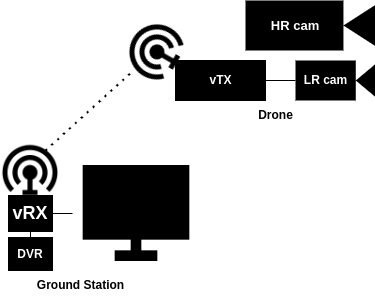
\includegraphics[scale=0.5]{figures/recording_schematics_2.png}
  \caption{Structure of the recording scheme}
  \label{img:recordin_schematics}
\end{figure}
To capture LR frames we used a CADDXFPV Ratel2 Analog Camera \cite{caddx}. As shown in Figure \ref{img:recordin_schematics}, the camera is connected to a 5.8Ghz video transmitter (vTX) that streams the signal to a receiver (vRX) on the ground, the receiver is connected to the navigation screen and also to the DVR (Digital Video Recorder) that saves the video stream on an SD card. While the camera itself can capture 1200TVL the color encoding conversion standard in use is PAL \cite{pal} so, according to the specifications, once recorded via DVR the resolution of the video is  \(720\times576\) and the frame rate 25 frames per second.

Another major difference between the two cameras is the field of view, respectively 120° for the Runcam and 165° for the Ratel2. This is due a a different combination of lens and sensor size, and results in two widely different video streams with a great amount of distortion. Before running any kind of training both images must be rectified and the content of each frame must overlap with the one recorded and the other camera. The cameras' properties are shown side-by-side in Table \ref{tab:cam_table}.






\begin{table}[h]
\centering
\caption{Resulting video streams}
\label{tab:cam_table}
\begin{tabular}{l|l|l|l|l|}
  \cline{2-5}
                                        & \cellcolor[HTML]{C0C0C0}Resolution {[}px{]} & \cellcolor[HTML]{C0C0C0}Aspect Ratio & \cellcolor[HTML]{C0C0C0}Frame rate {[}fps{]} & \cellcolor[HTML]{C0C0C0}Field of View {[}°{]} \\ \hline
  \multicolumn{1}{|l|}{Runcam 2}        &  \(1920\times1080\)                                   & 16:9                                 & 60                                           & 120                                           \\ \hline
  \multicolumn{1}{|l|}{CADDXFPV Ratel2} &  \(720\times576\)                                     & 4:3                                  & 25                                           & 165                                           \\ \hline
  \end{tabular}
\end{table}





\section {Camera Calibration}
\label{sec:camera_calib}

To perform camera calibration it has been decided to use the OpenCV library \cite{opencv}, which offers a large set of powerful modules for image manipulation and computer vision, among all the others, its pinhole camera model has all the tools to efficiently perform calibration and rectification.

\begin{figure}[h]
  \centering
  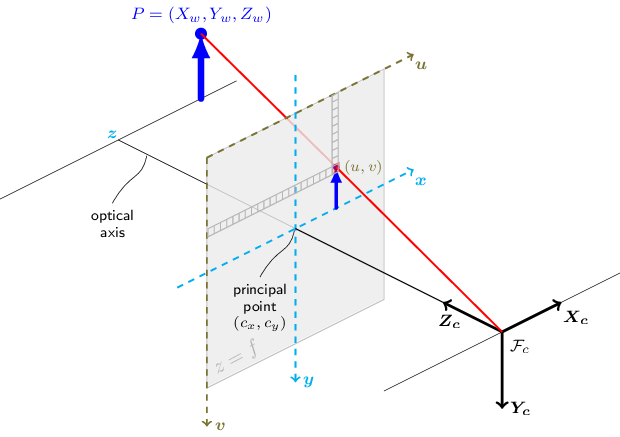
\includegraphics[scale=0.3]{figures/pinhole.png}
  \caption{Illustration of the pinhole camera model.}
  \label{img:pinhole_img}
\end{figure}

The pinhole camera model describes the mathematical relationship between the coordinates of a point in three-dimensional space and its projection onto the image plane of an ideal pinhole camera, where the camera aperture is described as a point and no lenses are used to focus light \cite{wikipinhole}.
The distortion-free projective transformation given by a pinhole camera model is shown below.

\[s \; p = A \begin{bmatrix} R|t \end{bmatrix} P_w,\]

Where \(P_w\) is a 3D point expressed with respect to the world coordinate system, \(p\) is a 2D pixel in the image plane, \(A\) is the camera intrinsic matrix, \(R\) and \(t\) are the rotation and translation that describe the change of coordinates from world to camera coordinate systems (or camera frame) and \(s\) is the projective transformation's arbitrary scaling and not part of the camera model \cite{opencvcalib}.

The camera intrinsic matrix \(A\) (Figure \ref{fig:camera_matrix}) projects 3D points given in the camera coordinate system to 2D pixel coordinates, it's composed of the focal lengths \(fx\) and \(fy\), which are expressed in pixel units, and the principal point (\(cx\),\(cy\)), that is usually close to the image center \cite{opencvcalib} \cite{888718}.

\begin{figure}[h]
\caption{Intrinsic camera matrix}
\label{fig:camera_matrix}
\[A = \left (
  \begin{array}{ c c c}
  f_x & 0   & c_x \\
   0  & f_y & c_y \\
   0  & 0   & 1 \\
  \end{array}
\right )\]
\end{figure}


The intrinsic camera matrix is not the only set of parameters estimated during the calibration process. Real lenses introduce, to some degree, barrel distortion and tangential distortion, to compensate for this, a vector of distortion coefficients is estimated along the intrinsic camera matrix and subsequently used in all the applications of the model.\newline


The estimation algorithm is based on the implementations presented in  \cite{888718} and \cite{matlab}: several pictures of a calibration pattern of known geometry are taken from different positions, for each view of the pattern the algorithm computes the intrinsic parameters, after that the camera position in respect to the calibration pattern is estimated using solvePnP \cite{opencvsolvepnp}. The last step is to run the Levenberg-Marquardt optimization algorithm to minimize the reprojection error (sum of the square distances between the observed features on the calibration pattern and the estimated position of said feature reprojecting the 3D object point on the visual plane).

Most of the time a chessboard pattern is enough to perform this kind of calibration, however, OpenCV's \emph{findChessboardCorners} function only detects the pattern when the entire board is in frame, this means that the detection fails most of the time when the board is moved to the corners of the screen, which is exactly where the distortion is more pronounced. For this reason, a ChArUco board has been used instead.

\begin{figure}[h]
  \centering
  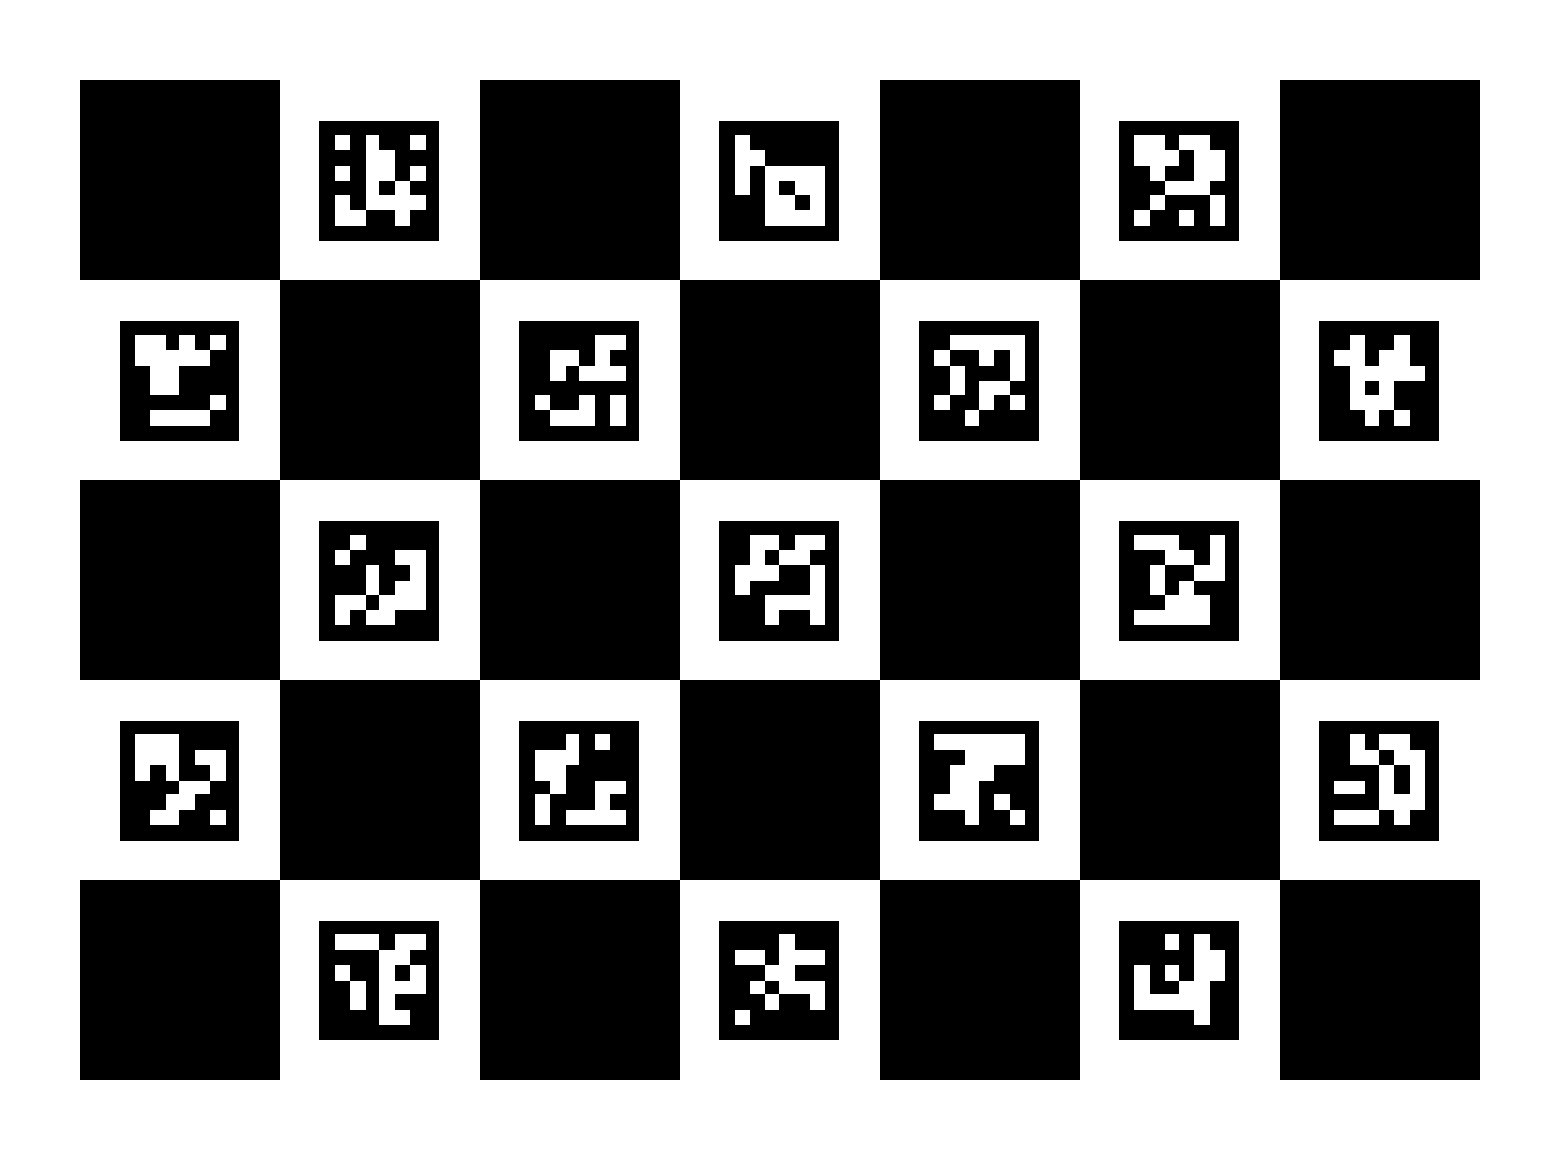
\includegraphics[scale=0.15]{figures/charucoboard.png}
  \caption{ChArUco board used for the calibrations.}
  \label{img:ch_board}
\end{figure}

The ChArUco board (Figure \ref{img:ch_board}) incorporates a standard chessboard pattern with a set of ArUco markers for detection, this allows the algorithm to detect the unique labels and from that it extrapolates the exact position of each pattern corner even if the board is only partially visible. Each pattern corner is first refined at a sub-pixel level for better accuracy, and after that, all the detected corners are paired, as 2D coordinates, to the 3D points in the calibration pattern frame of reference.

The quality of the board used for calibration is extremely important for proper parameter estimation, paper or plastic boards can introduce imperceptible deformations that can seriously tarnish the results of the process, on top of that temperature and humidity changes can cause the board to contract or dilate, thus a flat tv screen has been used to run the calibration for both cameras, ensuring a leveled plane and uniform illumination on the entire surface. Another reason to choose a big TV screen over a printed pattern is that the low resolution of the LR camera makes the detection of the ArUco markers difficult.

\begin{figure}[h]
  \centering
  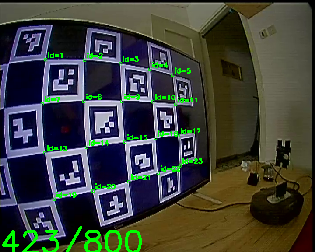
\includegraphics[scale=0.7]{figures/not_all.png}
  \caption{Frame taken during the calibration process. It shows how, even if the pattern is only partially visible, the corners are successfully detected and labeled with the correct ID.}
  \label{img:ch_calib}
\end{figure}

To ensure precise calibration results a flat pattern is appropriate, but not enough. The algorithm needs hundreds of data points over the span of tenths of images, it's important to make sure that the images cover a large volume of angles with respect to the target and, ideally, that they are distributed uniformly in the set. In order to follow these constraints closely and to keep the process as repeatable as possible without making it too time-consuming, the calibration pipeline has been divided into two parts that can be run together: datapoints capture and intrinsic parameters estimation.

During the datapoints capture, the script is fed a video taken from one of the two cameras, panning around the calibration pattern, slowly to avoid vibrations and motion blur, and progressively covering the entire camera frame from various angles and distances. A frame is considered valid when the number of detected corners is higher than a threshold set in advance, this is to make sure that even when part of the board is not visible (i.e. close to the corners) data is collected but if too few corners are detected (i.e. due to sudden movements or distance) the data is considered bad and the frame discarded.

Once enough valid frames have been captured a number of those data points is randomly sampled from the pool and fed to the camera calibration function that calculates the intrinsic camera matrix and the distortion coefficients vector. As hinted in the chapter introduction this kind of calibration is an optimization problem, in particular, the optimizer tries to minimize the RMS reprojection error, which is the square distance of the pattern keypoints detected on the image and the same points reprojected on the image using the calibrated camera model. This distance is expressed in pixels and typically one should expect to get values around 1.

A larger amount of images does not necessarily mean a better result and also the level of the threshold has a big impact on the quality of the calibration, it's a tradeoff between giving the algorithm more datapoints around the frame edges and dropping points that might affect negatively the process.

\begin{figure}[H]
  \centering
  \begin{subfigure}{.5\textwidth}
    \centering
    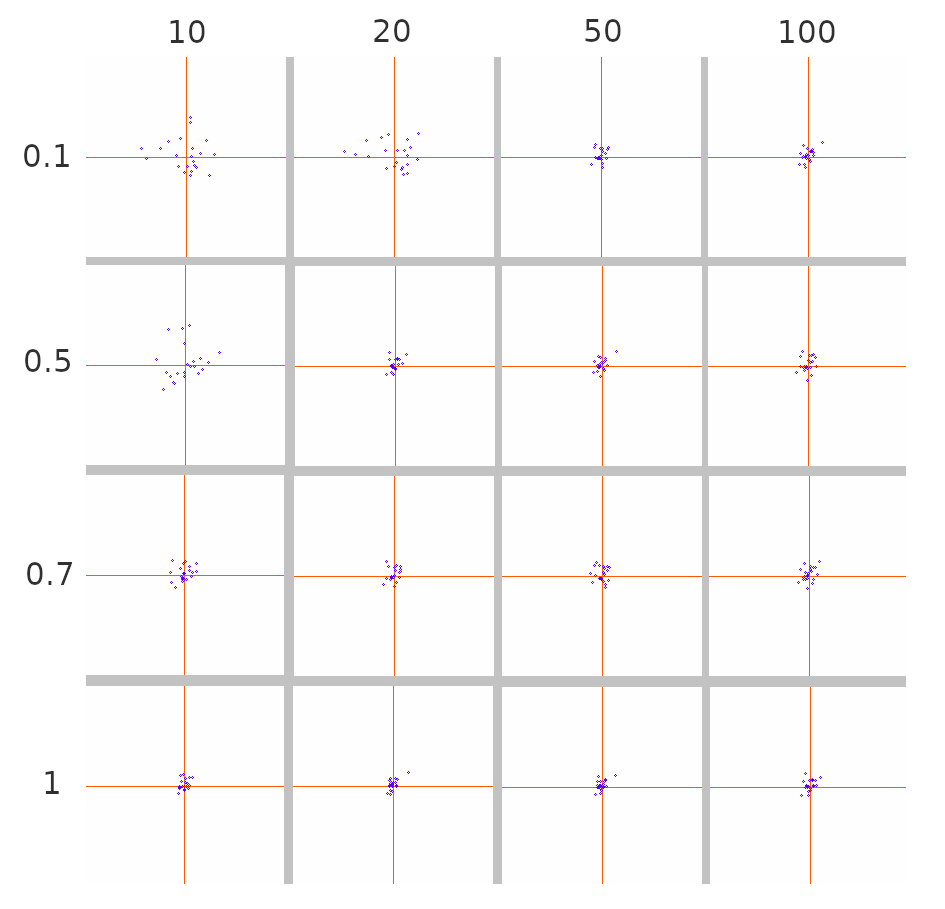
\includegraphics[width=.8\linewidth]{figures/reprj_dist_LR.png}
    \caption{Distribution of reprojection errors with
    \newline respect to number of samples and threshold.}
    \label{fig:reprj_dist_LR}
  \end{subfigure}%
  \begin{subfigure}{.5\textwidth}
    \centering
    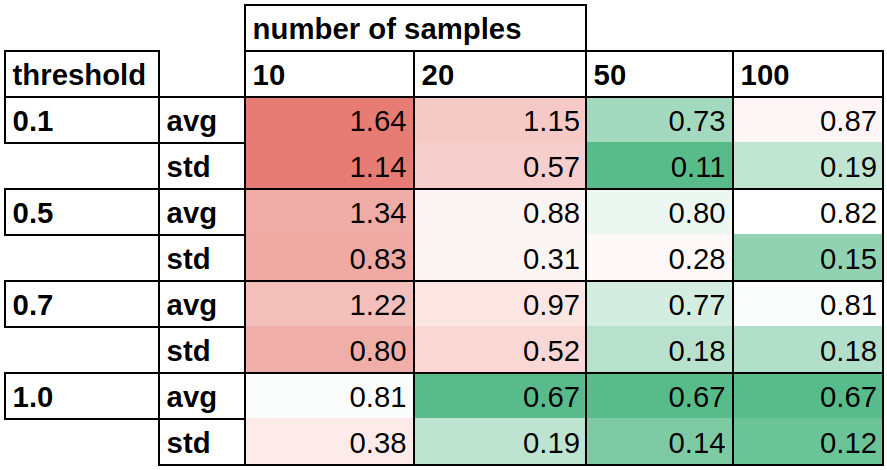
\includegraphics[width=0.8\linewidth]{figures/calib_results_table_LR.png}
    \caption{RMS reprojection error averaged over 20 calibrations and standard deviation with respect to number of samples and threshold.}
    \label{fig:calib_stats_LR}
  \end{subfigure}
  \caption{Analysis of the calibration results with the LR camera.}
  \label{fig:calib_analysis_LR}
\end{figure}

\begin{figure}[H]
  \centering
  \begin{subfigure}{.5\textwidth}
    \centering
    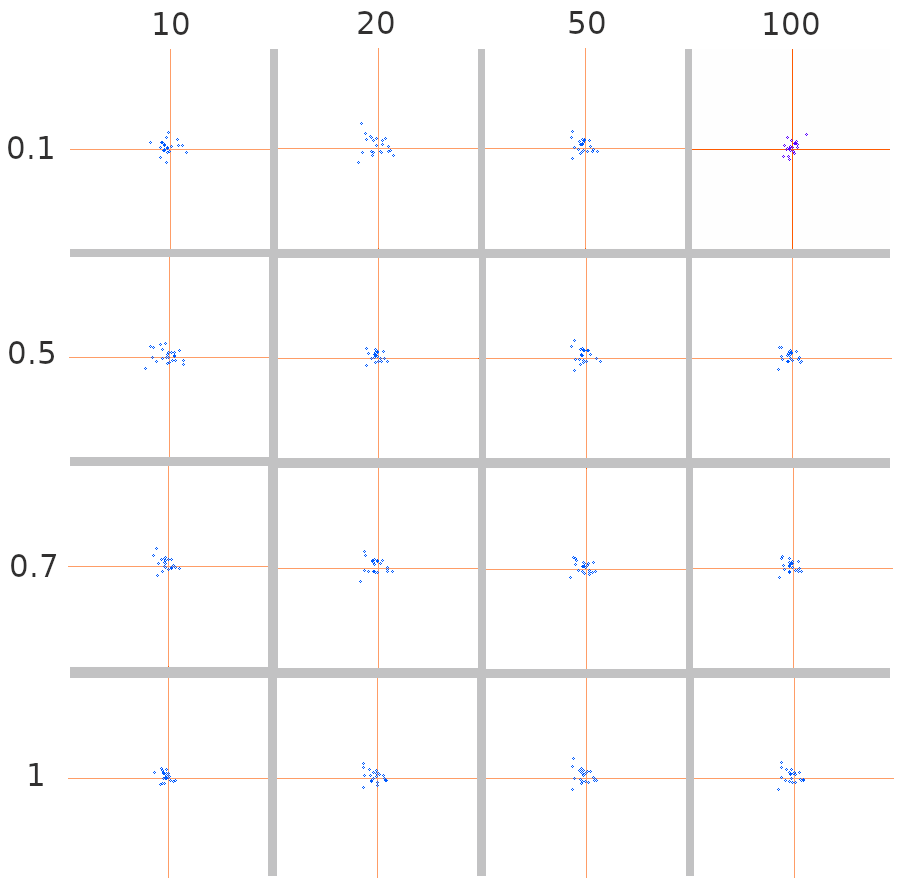
\includegraphics[width=.8\linewidth]{figures/reprj_dist_HR.png}
    \caption{Distribution of reprojection errors with
    \newline respect to number of samples and threshold.}
    \label{fig:reprj_dist_HR}
  \end{subfigure}%
  \begin{subfigure}{.5\textwidth}
    \centering
    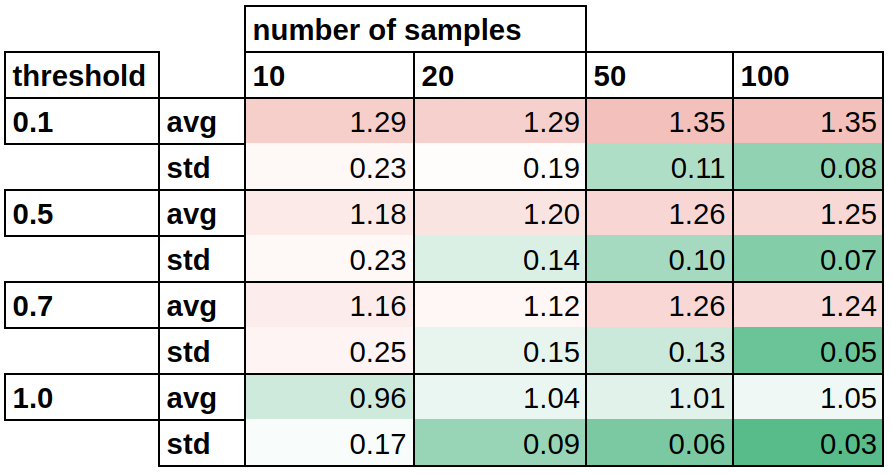
\includegraphics[width=0.8\linewidth]{figures/calib_results_table_HR.png}
    \caption{RMS reprojection error averaged over 20 calibrations and standard deviation with respect to number of samples and threshold.}
    \label{fig:calib_stats_HR}
  \end{subfigure}
  \caption{Analysis of the calibration results with the HR camera.}
  \label{fig:calib_analysis_HR}
\end{figure}
The analysis in Figures \ref{fig:calib_analysis_LR} and \ref{fig:calib_analysis_HR} have been done separately for the low-res camera and the high-res camera. For consistency, it's been used a single video from each camera and a total of around 600 calibrations were run before averaging for each combination of thresholds and amount of frames used.

Figure \ref{fig:calib_stats_LR} and Figure \ref{fig:calib_stats_HR} show how, for both cameras, there's a strong correlation between the number of samples used in each calibration and the consistency of the inaccuracies, as the standard deviation shrinks with the number of datapoints. The averaged error doesn't always follow the same pattern, however, it's safe to assume that if it doesn't fluctuate excessively, a larger set of corners guarantees a better generalization of the camera model. Also, higher thresholds generally yield better results as single frames contain more correlated points, unfortunately, this leads to less information about the distortion around the edges of the image to be examined. Generally, a low error on a higher threshold can be misleading as it indicates that the approximation of the camera model is good taking into consideration mostly images that fit inside the entire frame, so around the middle where distortion is present the least.

A second factor to take into consideration is the distribution of errors, RMS reprojection error only gives information about the averaged distance between detected and reprojected points without taking into account their direction. Figures \ref{fig:reprj_dist_LR} and \ref{fig:reprj_dist_HR} show how for each combination of threshold and number of samples the reprojected points differ from their detected position on the two axes, a good calibration will show a cloud of datapoints distributed uniformly around the origin, if the spread it skewed in one direction that might be the symptom of a poor estimation or bad measurements. It's worth mentioning that these kinds of off-center patterns are not evident from the RMS error reading alone so it's good practice to run a specific check for these particular occurences.

The final calibrations used for this dataset had RMS reprojection errors of, respectively, 0.67px for the low-resolution camera and 0.98px for the high-resolution camera. Once obtained the intrinsic camera matrix and the distortion coefficients vector it's enough to pass them and the distorted image as parameters to OpenCV's \emph{undistort} function to get the rectified results.

\begin{figure}[H]
  \centering
  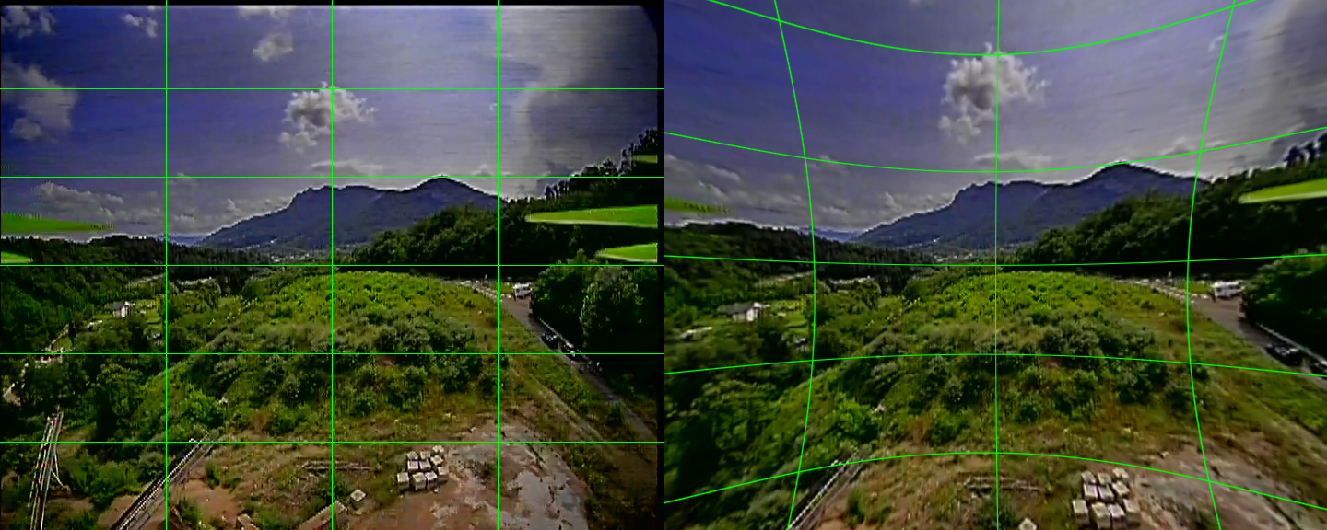
\includegraphics[width=1\textwidth]{figures/bef_aft_rect.png}
  \caption{The same image before and after rectification.}
  \label{img:rectify_sbs}
\end{figure}

Figure \ref{img:rectify_sbs} shows side by side the rectification result, a grid overlay has been added to highlight how the image gets distorted in the process. It's easy to see how part of the original image is lost due to the fact that, while all the pixels are geometrically transformed to their new position, the image shape is kept the same. Now that the distortion is removed it's possible to move to the next step where LR and HR pairs are aligned.

\section{Temporal Alignment}
\label{sec:temp_align}

The temporal alignment process is rather simple: find a pair of frames taken at the same instant and use them as a point of reference to navigate in a synchronized way through the videos.

The two cameras are not wired one to the other so while it's not possible to get perfect synchronization it's feasible to extrapolate a good enough approximation that can be refined further processing the images. The first step is to find two frames that are as close as possible, to achieve this in the first few seconds of every clip an external timer is recorded by both cameras, afterward, in post processing both clips are shown side by side and, manually, a pair of frames is chosen as reference and the frame indexes are saved in the corresponding clips folder.

\begin{figure}[H]
  \centering
  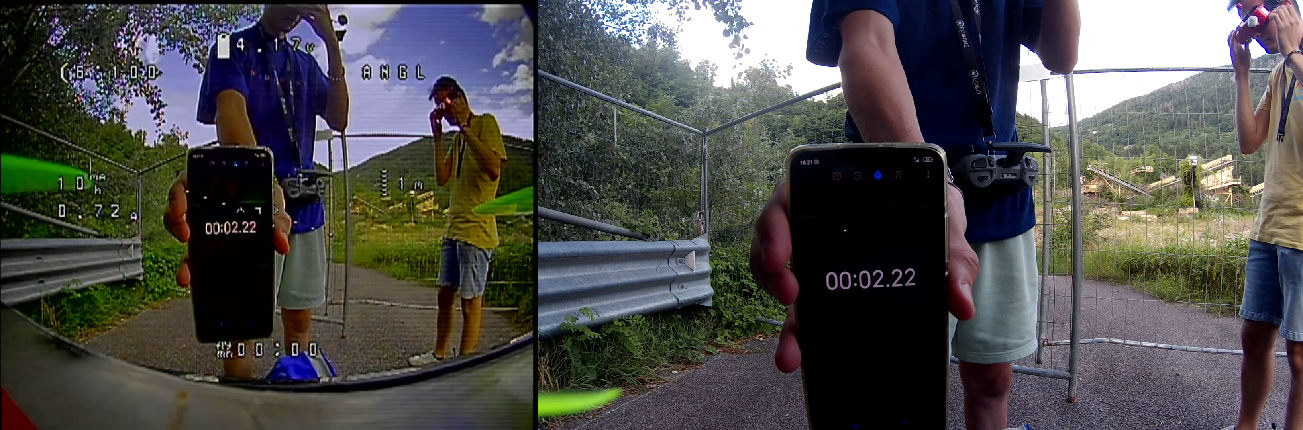
\includegraphics[width=0.8\textwidth]{figures/time_sync_kp.png}
  \caption{Videos are shown side by side and it's possible to move independently frame by frame until a correspondence is found.}
  \label{img:time_sync}
\end{figure}

Once the reference point is found it's clear from Figure \ref{img:temp_align} that's just not possible to move frame by frame and expect the video to stay synchronized, moreover, only one every few frames will align like the reference pair. In this specific case, the framerates being 25 for the low resolution and 60 for the high resolution implies that one pair every 5 LR frames and 12 HR frames will have the same alignment thus it's been decided to keep one frame every 200ms. While it might seem like a waste it actually solves the problem of having too many similar frames with redundant information.

It should be emphasized that since the cameras are not physically synchronized and the shutter speeds are different it's just not possible to get perfect matches, the next steps try to tackle this problem with some image manipulation in post-processing.

\section{Spatial Alignment}
\label{sec:spatial_align}

The two cameras have widely different AFOVs, so it's clear that the images, as they come out of the rectification and synchronization, depict two much different sections of the world, on top of that, even if the cameras are fixed in place and point to the same direction it can't be taken for granted that the mounting positions are aligned to the degree of precision needed to create a practical dataset.

The first step of the spatial alignment is to geometrically transform one of the two images so that the content of both overlaps, this is done manually, it's important to do it separately for each pair of clips: landing, moving the drone around, removing and inserting the SD cards in the camera, all the mentioned actions can cause small movements of the cameras that render any alignment done beforehand, useless.

\begin{figure}[H]
  \centering
  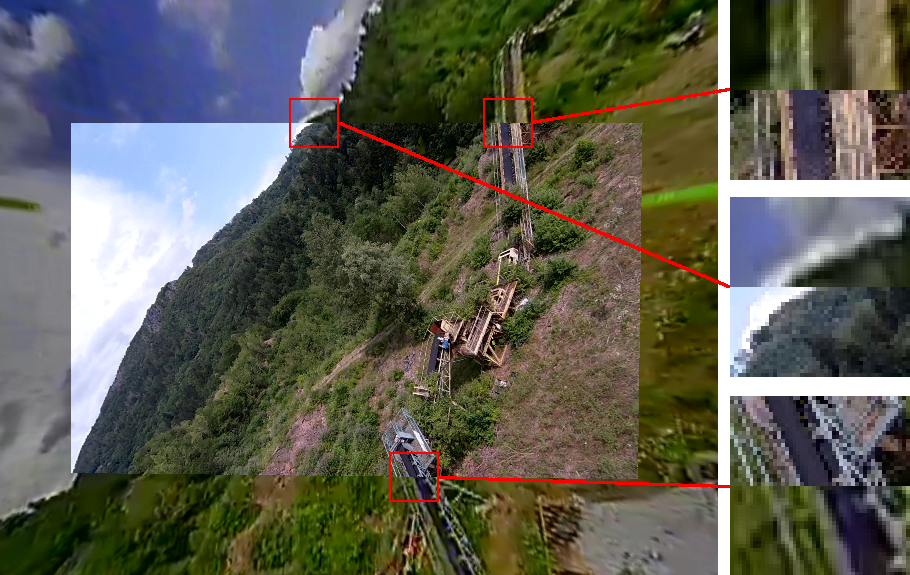
\includegraphics[width=0.7\textwidth]{figures/HR_on_LR_M_err_highlight.png}
  \caption{Sharp turns and sudden movements make the small misalignments more evident. Here the HR frame is overlapped to the LR one to fit the same world area using only the manual alignment.}
  \label{img:align_err}
\end{figure}

The manual procedure consists in showing the user a set of pairs of LR and HR frames side by side, the user will then proceed to select, by clicking on the two images, pairs of pixels that represent the same exact area in both frames. Once around 20 pairs have been selected the script can estimate the affine transform matrix that will be used in the initial alignment of all the frame pairs of that specific clip.

As mentioned in the introduction both cameras are fixed in place and point in the same direction, despite that the aerial platform is not devoid of a copious amount of vibrations caused by turbulences and by the four motors spinning at tens of thousands of rounds per minute.
This causes small, almost imperceptible, movements in the cameras that only come apparent in post-production as shown in figure \ref{img:align_err}, this, in addition to the inevitably small discrepancies in the synchronization of frames, calls for an alignment solution based solely on the content of the single image pairs. Two solutions have been implemented to solve this issue, they offer their pros and cons and both can be used interchangeably or combined.


\subsection {Feature Matching}
\label{subsec:feature_match}

Feature matching refers to the act of recognizing features of the same object across images with slightly different viewpoints \cite{feat_match}. If enough keypoints are correctly detected and paired between the two frames it's possible to use a procedure similar to the initial alignment and automatically refine the position of the low-resolution image with regard to the high resolution one.

Three techniques have been chosen and tested on the dataset directly using their OpenCV implementation with some small changes to their criteria \cite{6126544, lowe1999object, 6809191, DBLP:journals/corr/abs-1710-02726}:

\begin{itemize}
  \item \textbf{ORB}\newline
  The ORB (Oriented FAST and Rotated BRIEF) algorithm is a sophisticated integration of the FAST keypoint detection and BRIEF descriptor techniques, supported by modifications for heightened performance. ORB begins by employing the FAST algorithm to detect keypoints, followed by applying the Harris corner measure to select the most significant keypoints from this set. Notably, FAST lacks orientation determination and is sensitive to rotation; however, ORB addresses this by utilizing the computed centroid of the patch surrounding a corner, its orientation determined by the vector from corner to centroid, supplemented by moment calculations for improved rotation invariance. In dealing with the limitation of BRIEF descriptors under in-plane rotations, ORB computes a rotation matrix based on patch orientation before adapting the descriptors accordingly. This intricate alignment refines the descriptors' performance, resulting in an algorithm that excels in various computer vision tasks by harmonizing FAST-based keypoints and orientation-aware BRIEF descriptors \cite{6126544}.
  \item \textbf{SIFT}\newline
  Lowe's Scale-Invariant Feature Transform (SIFT) presents a comprehensive solution to challenges such as image rotation, affine transformations, intensity variations, and changes in viewpoint during feature matching. The SIFT algorithm is structured around four fundamental steps. Firstly, it estimates scale space extrema by employing the Difference of Gaussian (DoG) approach. Subsequently, it engages in key point localization, identifying and refining potential key point candidates while eliminating low-contrast points. Thirdly, a key point's orientation is determined by leveraging local image gradients. Lastly, the algorithm generates descriptors for each key point by computing local image descriptors based on gradients' magnitude and orientation, encapsulating essential information for subsequent matching processes \cite{lowe1999object}.
  \item \textbf{SIFT with FLANN based matcher}\newline
  FLANN (Fast Library for Approximate Nearest Neighbors) stands as a versatile tool designed to facilitate rapid and approximate searches for nearest neighbors within spaces characterized by high dimensionality. Within its framework, a set of algorithms has been curated, and meticulously selected for their performance in nearest-neighbor searches. Moreover, FLANN boasts an integrated mechanism for dynamically selecting the most fitting algorithm and optimal parameters, adapting to the specific dataset at hand and ensuring efficient and effective neighbor searches \cite{6809191}.
\end{itemize}

Working with automated feature matching poses the risk of detecting false positives that negatively affect the resulting transformation. OpenCV's \emph{findHomography} solves this problem using RANSAC to find end exclude outliers while estimating the affine transform, nevertheless, it was key to refine as much as possible the feature match trading off datapoints for cleaner and more precise measurements.
Testing revealed that on this task SIFT performed much better compared to ORB, the addition of a FLANN matcher further improved the precision of the algorithm generating decent, albeit not perfect, results (Figure \ref{img:deep_match}).

\begin{figure}[H]
  \centering
  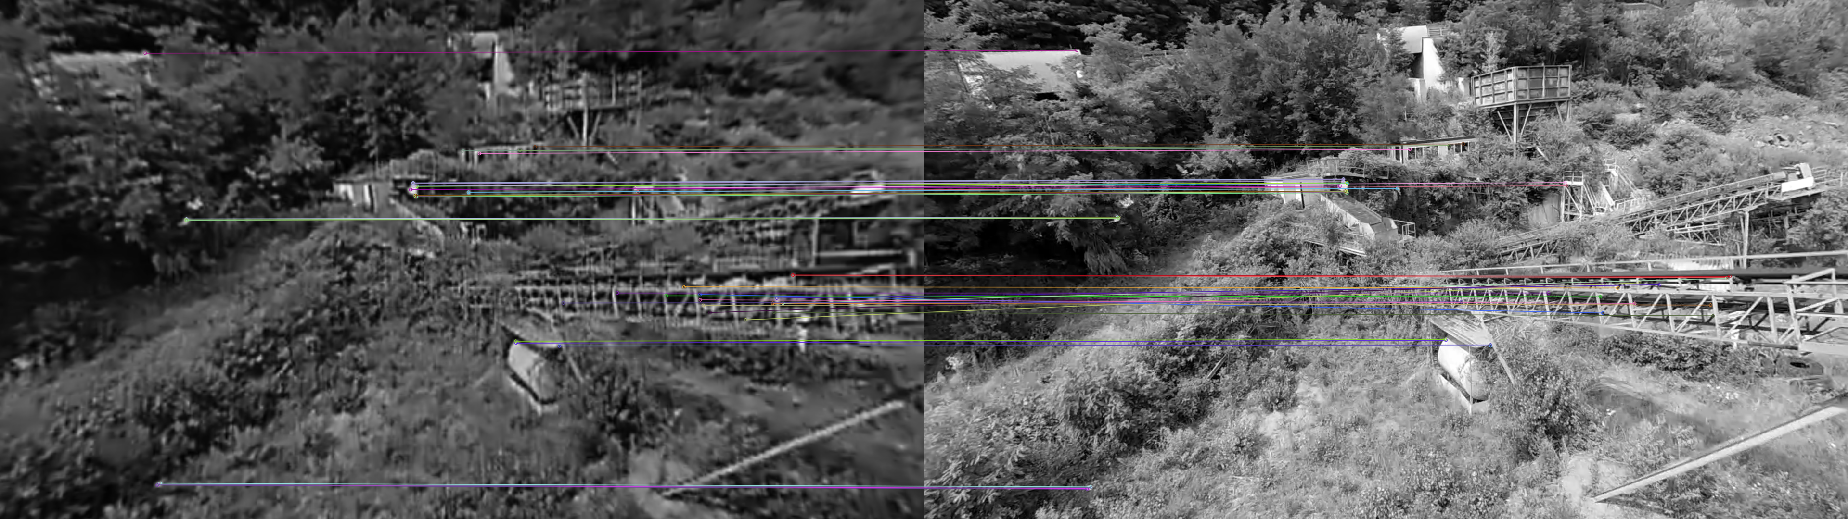
\includegraphics[width=1\textwidth]{figures/ORB.png}
  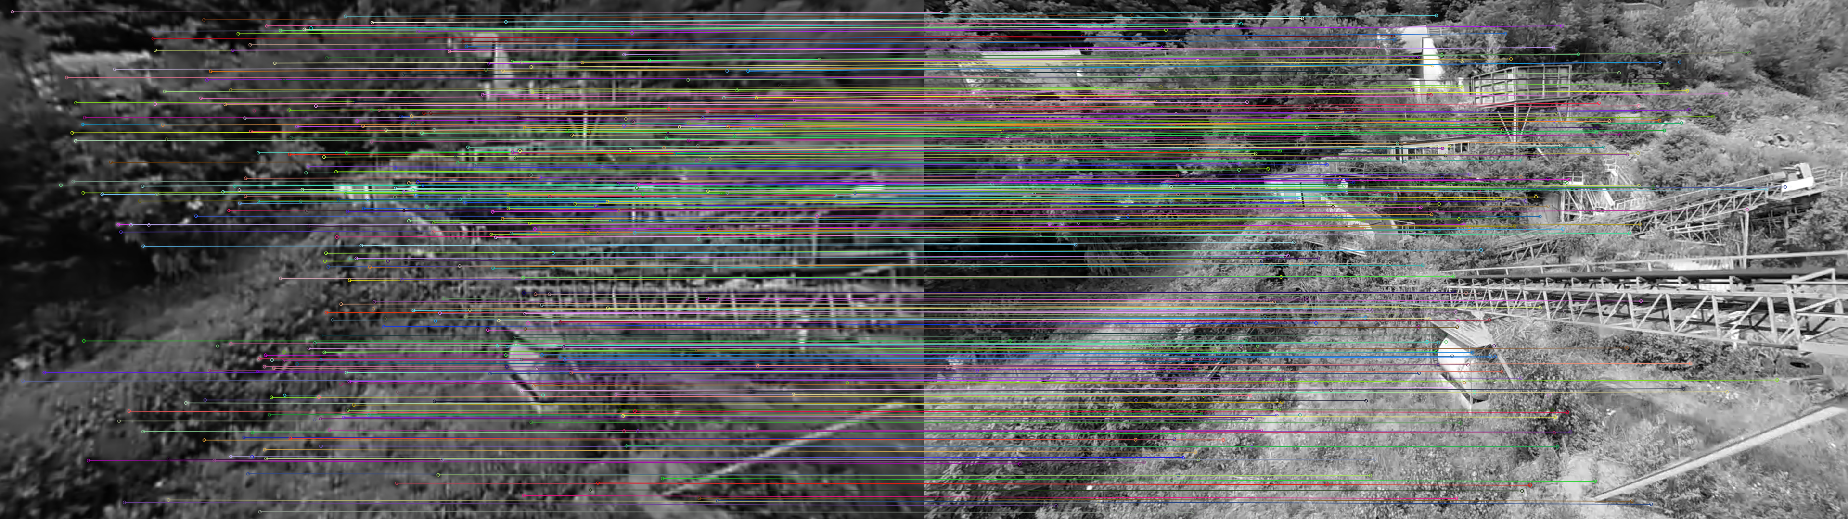
\includegraphics[width=1\textwidth]{figures/SIFT.png}
  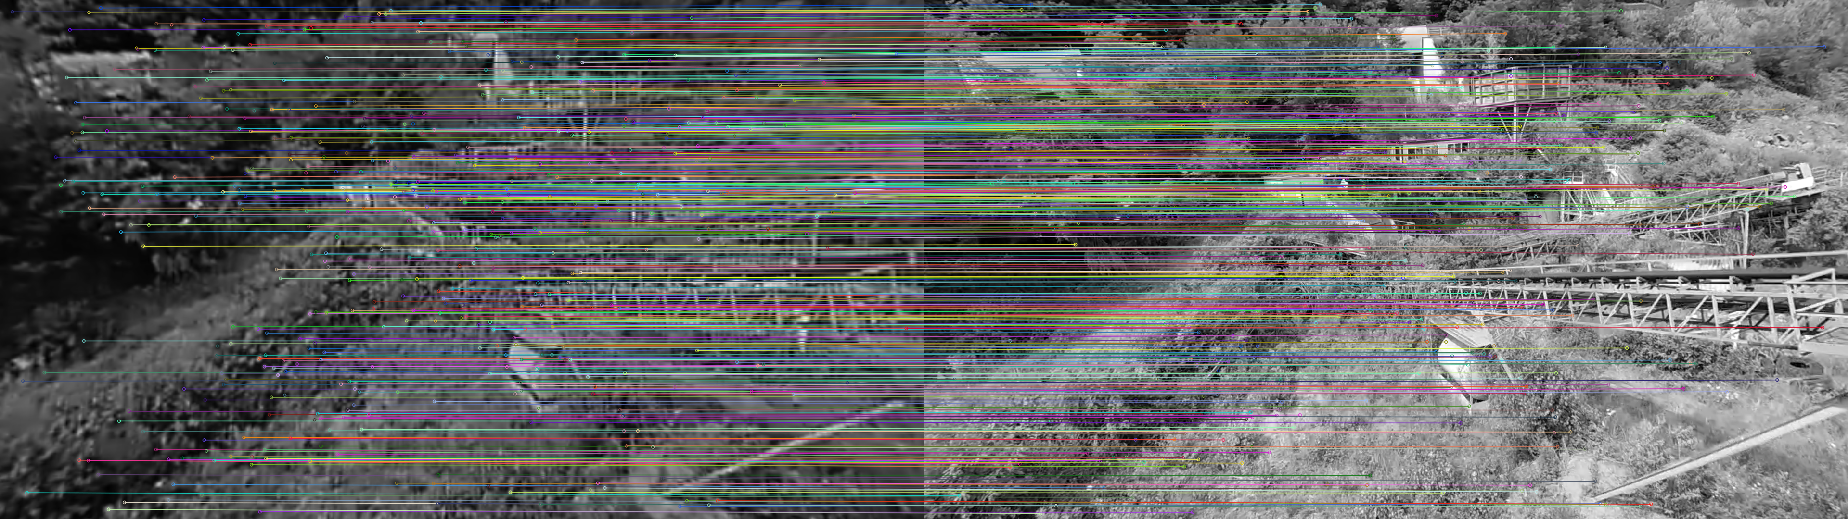
\includegraphics[width=1\textwidth]{figures/FLANN.png}
  \caption{In order, ORB, SIFT, SIFT with FLANN. While keeping the same constraints for all three approaches, using SIFT with FLANN matcher resulted in many more and much more consistent datapoints.}
  \label{img:orb_sift}
\end{figure}

Some of the additional criteria include making sure that the keypoint's coordinates don't differ for more than a certain threshold (set between 5 and 20 pixels) between the two images and that keypoints are distributed uniformly on the image for better estimation of the affine transform matrix, otherwise, the frames are discarded. Needless to say running this whole procedure of, feature detection, feature matching, matrix estimation and perspective warp is a computationally expensive operation, taking several minutes for every batch of a few hundred images.

On top of that results are not as consistent as hoped, while most of the frames get correctly aligned, in some cases the estimation goes completely off rails resulting in severely warped frames scattered in the dataset. Although it's possible to just skim through the dataset and manually remove the affected images this is not a scalable solution when dealing with thousands of images.

\begin{figure}[H]
  \centering
  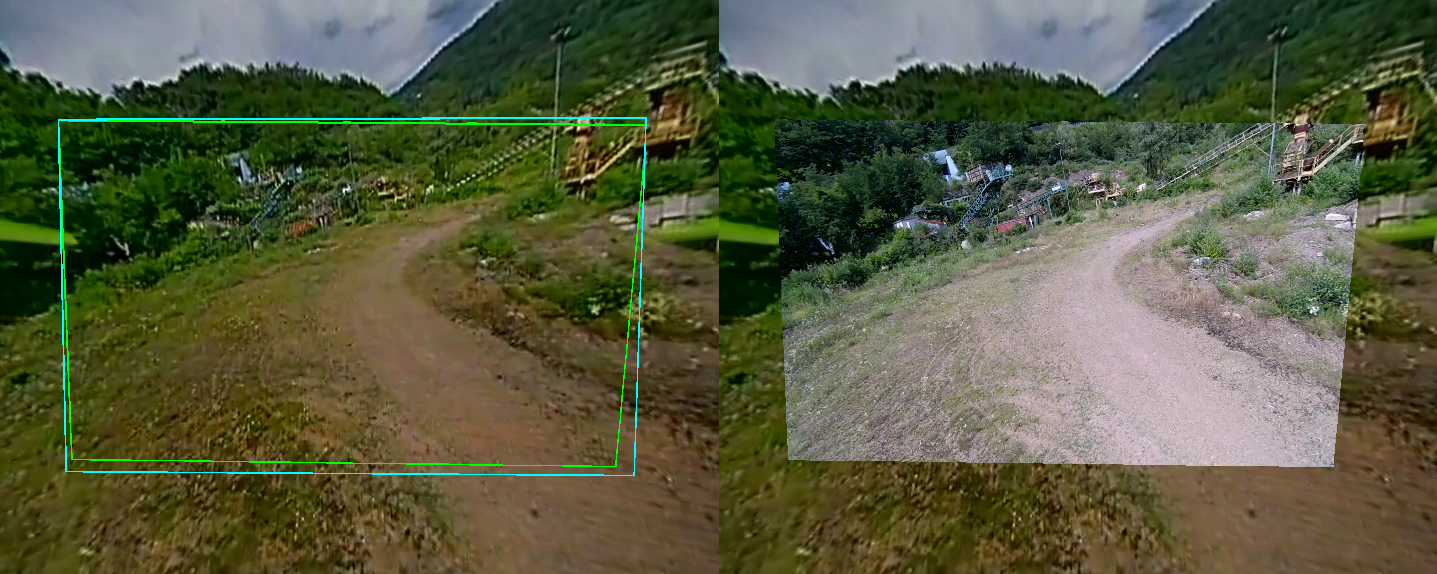
\includegraphics[width=1\textwidth]{figures/deep_match_sbs.png}
  \caption{The light blue rectangle represents how the HR frame fits in the LR frame using the initial clip alignment, the green rectangle is the fit of the HR image once the refined alignment procedure is run on this specific pair of frames. On the right is the final result. It must be noted that this image is just for reference, in the actual script the HR frame is left untouched to preserve its image quality, while the LR one endures all the warping and scaling.}
  \label{img:deep_match}
\end{figure}

\subsection {Template Matching}
\label{subsec:template_match}

Automatically verifying the quality of the alignment is not an easy task: if there was a metric to unequivocally define how precisely the two images match, that would be surely used in the alignment process itself. One could think to use template matching and, although the absolute value of the match doesn't say much when the images are so intrinsically different, it can effectively rank how close a set of low-resolution frames is compared to a high-resolution one.

This is the idea behind the second approach to spatial alignment. As mentioned before the non-perfect synchronization of frames (which is only possible if the two triggers are communicating or if one camera is shooting at a much higher framerate than the other) is a big factor when considering moving objects, which in this project is the case, but it can also be used to our advantage. The small offsets introduced by the camera movement over adjacent frames on a small window of time can actually compensate for the misalignments due to other factors.

For this approach instead of considering a single HR frame, every LR image is associated with a buffer of 5 high-resolution adjacent frames centered around the synchronized one and OpenCV's implementation of the \emph{matchTemplate} function is used to pick the one that most closely overlaps to the low-resolution image. Additionally \emph{matchTemplate} doesn't fare well with rotated targets, which is exactly what we are looking for as eventually a constrained version of the feature matching approach described in section \ref{subsec:feature_match} can be used to translate to the right position frames that match in orientation but not one the \(x\) and \(y\) axis.\newline

The function \emph{matchTemplate} works by moving a template around the image and giving for each position a score of similarity, for this reason, the template has to be smaller than the image and the size of the result will correspond to the room of movement of the top left pixel of the template, so it will look similar to a heatmap with the size of the difference of widths by the difference of heights.

For this reason, the templates, which are the HR frames, have to be cropped, and the crop will correspond to their wiggle room around the LR frame. Each cropped frame is run with the LR one in the \emph{matchTemplate} function and the pixel with the highest score is saved along its coordinates. Finally, the pixel with the highest score over the entire buffer is used to pick the frame that more closely matches the low-resolution one.

Ideally, if calibration, synchronization and alignment were perfect, when visualizing together the coordinates of the best pixel for each frame it would show a pattern corresponding to the movement of the camera and the best pick (the pixel with the highest score overall) should lay in the center, but obviously that's not always the case.

\begin{figure}[H]
  \centering
  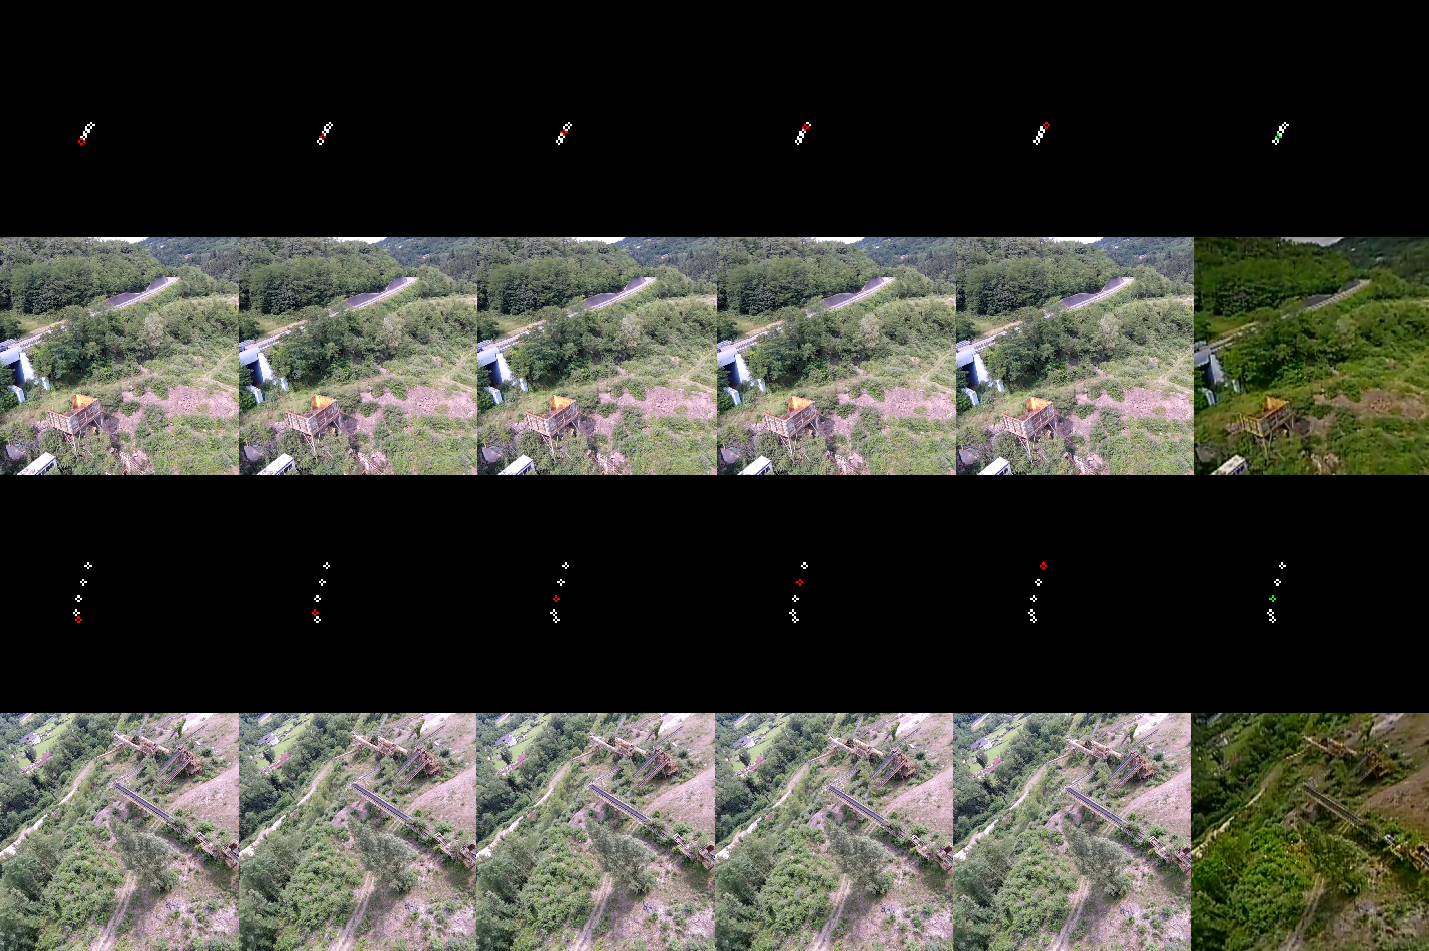
\includegraphics[width=0.7\textwidth]{figures/matchtemplate.png}
  \caption{Two different sequences of frames. On the bottom the buffer of 5 HR frames followed by the LR one. On the top the visualization of the coordinates of the best match for each frame, in red is highlighted the position of the frame below, in green is the highlighted the pixel that scored the highest overall.}
  \label{img:matchtempl}
\end{figure}

In Figure \ref{img:matchtempl} it's very clear the movement of the HR recording compared to the fixed LR frame. It's easy to see how the relative movement present in the buffer frames at the bottom is much faster than the one above as the points are more spread out. It's worth noting that the HR templates from size \(1920\times1080\) were cropped by 50 pixels on all sides, giving a squared wiggle room of side length 101px, also, the frame buffer of size 5 corresponds to about 8 milliseconds.

While, as mentioned before, it's possible to further refine the alignment by running the feature matching on top of the match template procedure it's been decided to ditch this extra step as the improvements to the dataset precision were marginal at the cost of increasing the computation time by an order of magnitude.

\section{Resulting Dataset}
\label{sec:final_dataset}

Once the spatial alignment is done the images are finally ready to be resized for the actual dataset. As an intermediate step, every frame is firstly cropped as a square and then resized to 1024 before being written to disk. The trainings were run with different images sizes, all smaller than  \(1024\times1024\), by storing them like this a lot of time is saved when creating different shaped dataset as the alignment doesn't need to be run again and the additional whole read, resize and write procedure takes just seconds even with thousands of images.


\begin{figure}[H]
  \centering
  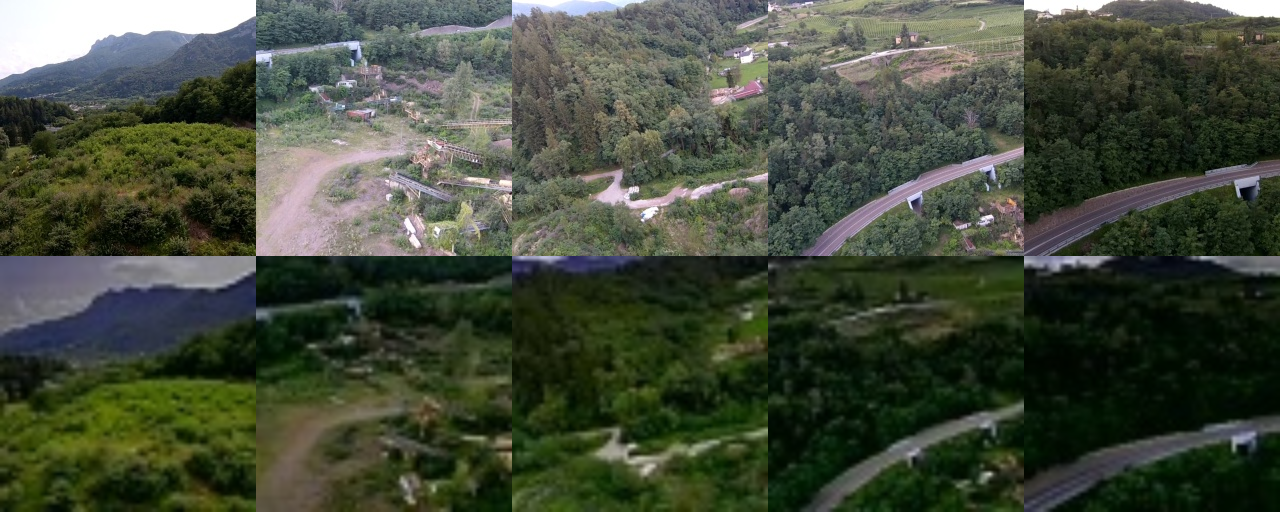
\includegraphics[width=1\textwidth]{figures/final_64_256.png}
  \caption{Samples from the 64 to 256 dataset.}
  \label{img:64_256}
\end{figure}

\begin{figure}[H]
  \centering
  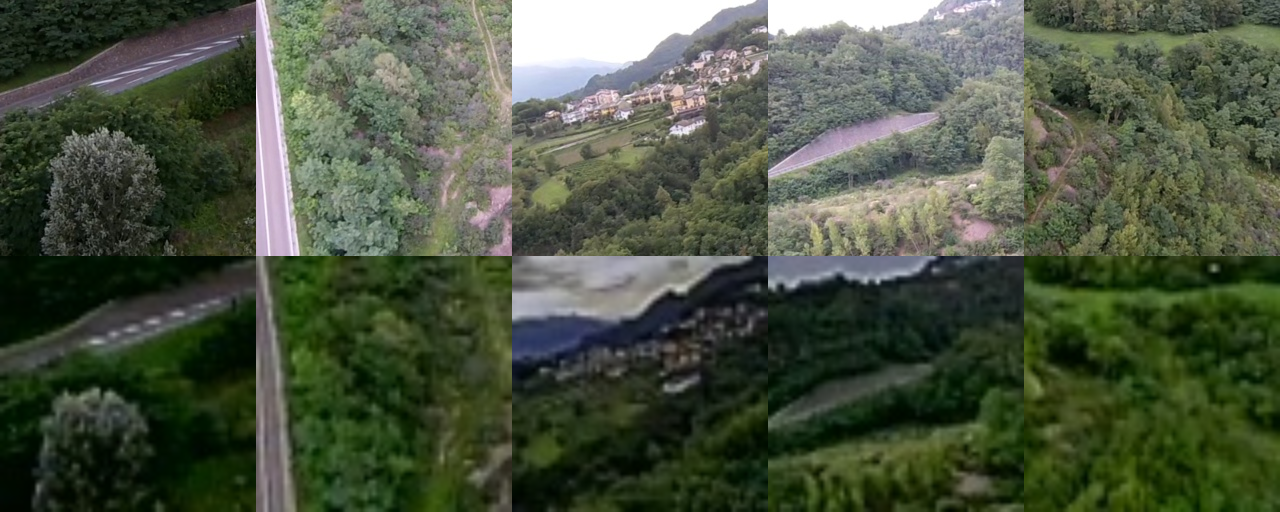
\includegraphics[width=1\textwidth]{figures/final_64_256_patches.png}
  \caption{Samples from the 64 to 256 patches dataset.}
  \label{img:64_256_p}
\end{figure}

\begin{figure}[H]
  \centering
  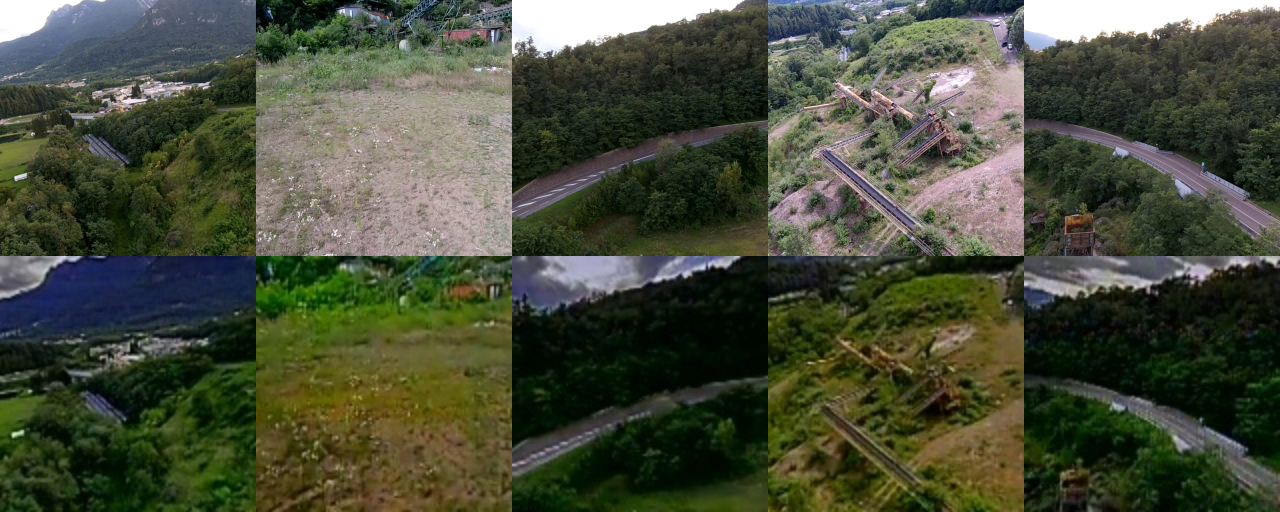
\includegraphics[width=1\textwidth]{figures/final_128_512.png}
  \caption{Samples from the 128 to 512 dataset.}
  \label{img:128_512}
\end{figure}


Although all the models were trained at x4 scale, to test the behavior of the networks with differently shaped datasets it's been chosen to use the following configurations:

\begin{itemize}
  \item  \(64\times64\) LR and  \(256\times256\) HR (Figure \ref{img:64_256})
  \item  \(64\times64\) LR and  \(256\times256\) HR patches splitting each frame into 4 squares (Figure \ref{img:64_256_p})
  \item  \(128\times128\) LR and  \(512\times512\) HR (Figure \ref{img:128_512})
\end{itemize}

The full size dataset is composed of 2459 images (2210 for training and 249 for validation), while the patches set is composed of 8652 images for training 624 for validation.
